\chapter{Microcontrollers Design}
\label{chap:microcontrollers-design}
\section{Introduction}
\label{sec:introduction}
Figure \ref{fig:microarchitecture} shows the microservices components that make up the design of \ac{RAILS}. The microservices,
highlighted with the light green colored background in Figure \ref{fig:microarchitecture} are shown connected to the \ac{IoT} components on the left side of the figure.
The \ac{IoT} components are the microcontrollers that are used to control the model railroad layout. The microcontrollers are connected to the \ac{MQTT} broker via Wi-Fi. 
The microcontrollers are programmed to provide model railroad sensors and actuators. A conceptual diagram of the microcontroller design is shown in Figure 
\ref{fig:system-concept} where the PC is the platform the \ac{MQTT} broker and the other microservices are running.
\begin{figure}[htbp]
    \centering
    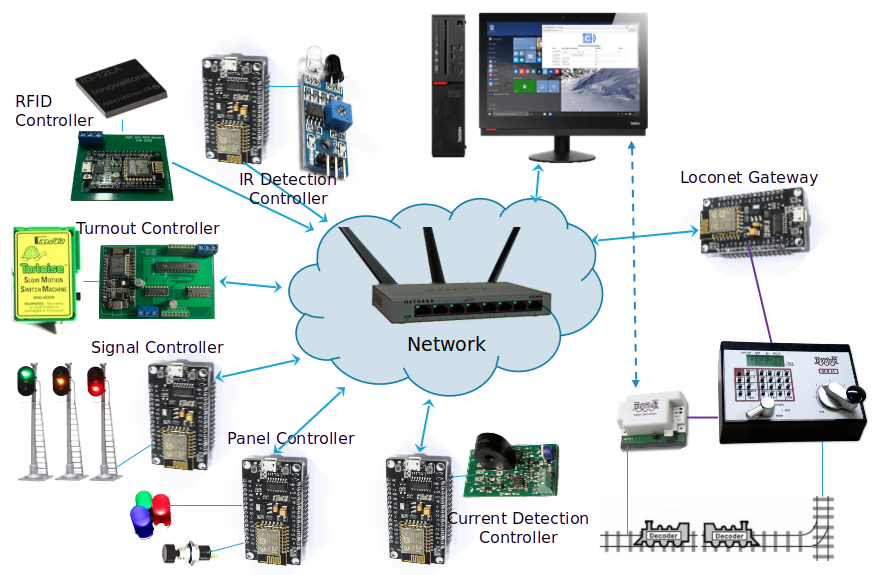
\includegraphics[scale=0.5]{system-concept.png}
    \caption{Components in the design of RAILS}
    \label{fig:system-concept}
\end{figure}

\section{Microcontrollers}
\label{sec:microcontrollers}
An ESP8266 development board is a small, breadboard-friendly circuit board that houses the ESP8266 Wi-Fi microcontroller chip along with additional components to make 
it easy to use for programming and prototyping. It's a popular choice for hobbyists and makers working on \ac{IoT} projects.
The key features of the ESP8266 are:
\begin{itemize}
\item 32-bit \ac{RISC} \ac{CPU}: Tensilica Xtensa LX106 running at 80 MHz
\item 64 KiB of instruction \ac{RAM}, 96 KiB of data \ac{RAM}
\item \ac{IEEE} 802.11 b/g/n \ac{Wi-Fi}
\item 16 \ac{GPIO} pins
\item \ac{SPI}, \ac{I2C}, \ac{I2S} interfaces with \ac{DMA} (sharing pins with \ac{GPIO})
\item \ac{UART} on dedicated pins
\item 1 10-bit \ac{ADC}
\item \ac{PWM} on all \ac{GPIO} pins with \ac{DMA} (sharing pins with \ac{GPIO})
\item 1 8-bit \ac{DAC}
\item 10 µA deep sleep current
\end{itemize}
The benefits of using an ESP8266 development board, such as the NodeMCU are:
\begin{itemize}
\item Breadboard-friendly
\item Versatile and easy to use
\item ESP8266 boards are some of the cheapest \ac{Wi-Fi} development boards available
\item Easy to program and debug, either with the Arduino \ac{IDE} or Visual Studio Code with PlatformIO.
\item Easy to connect to a network and the Internet
\end{itemize}

\section{RFID Microcontroller} 
\label{sec:rfid-microcontroller}
The RFID microcontroller is responsible for reading the \ac{RFID} tags attached to the rolling stock. The RFID microcontroller is programmed to:
\begin{itemize}
\item initializes \ac{Wi-Fi} and \ac{MQTT} paramters are set at compile time using values kept in a params.h file
\item connects to an \ac{MQTT} broker via \ac{Wi-Fi}
\item publishes info about this reader to the topic ``micros'' in the format: \\
\{``et'':``1590462747'',``sensor'':``rfidRdr01'',``msgType'':``initial'',``ip'':``192.168.0.19''\}
\item publishes a heartbeat to the topic ``micros'' in the format: \\
\{``et'':``1590462747'',``sensor'':``rfidRdr01'',``msgType'':``heartbeat''\}
\item reads values from a single ID-12LA or 7491E \ac{RFID} reader, formats the results as a \ac{JSON} string, 
gets Epoch time from an \ac{NTP} server and then publishes the \ac{JSON} String to the topic ``sensors/rfid''
in the format: \\
\{``et'':``1590463450'',``sensor'':``rfidRdr01'',``reader'':``1'',``rfid'':``1C0044CF23''\}
\end{itemize}

Figure \ref{fig:rfid-reader} depicts the circuit diagram of the RFID reader. The RFID reader is connected to the ESP8266 microcontroller via a serial connection.

\begin{figure}[htbp]
    \centering
    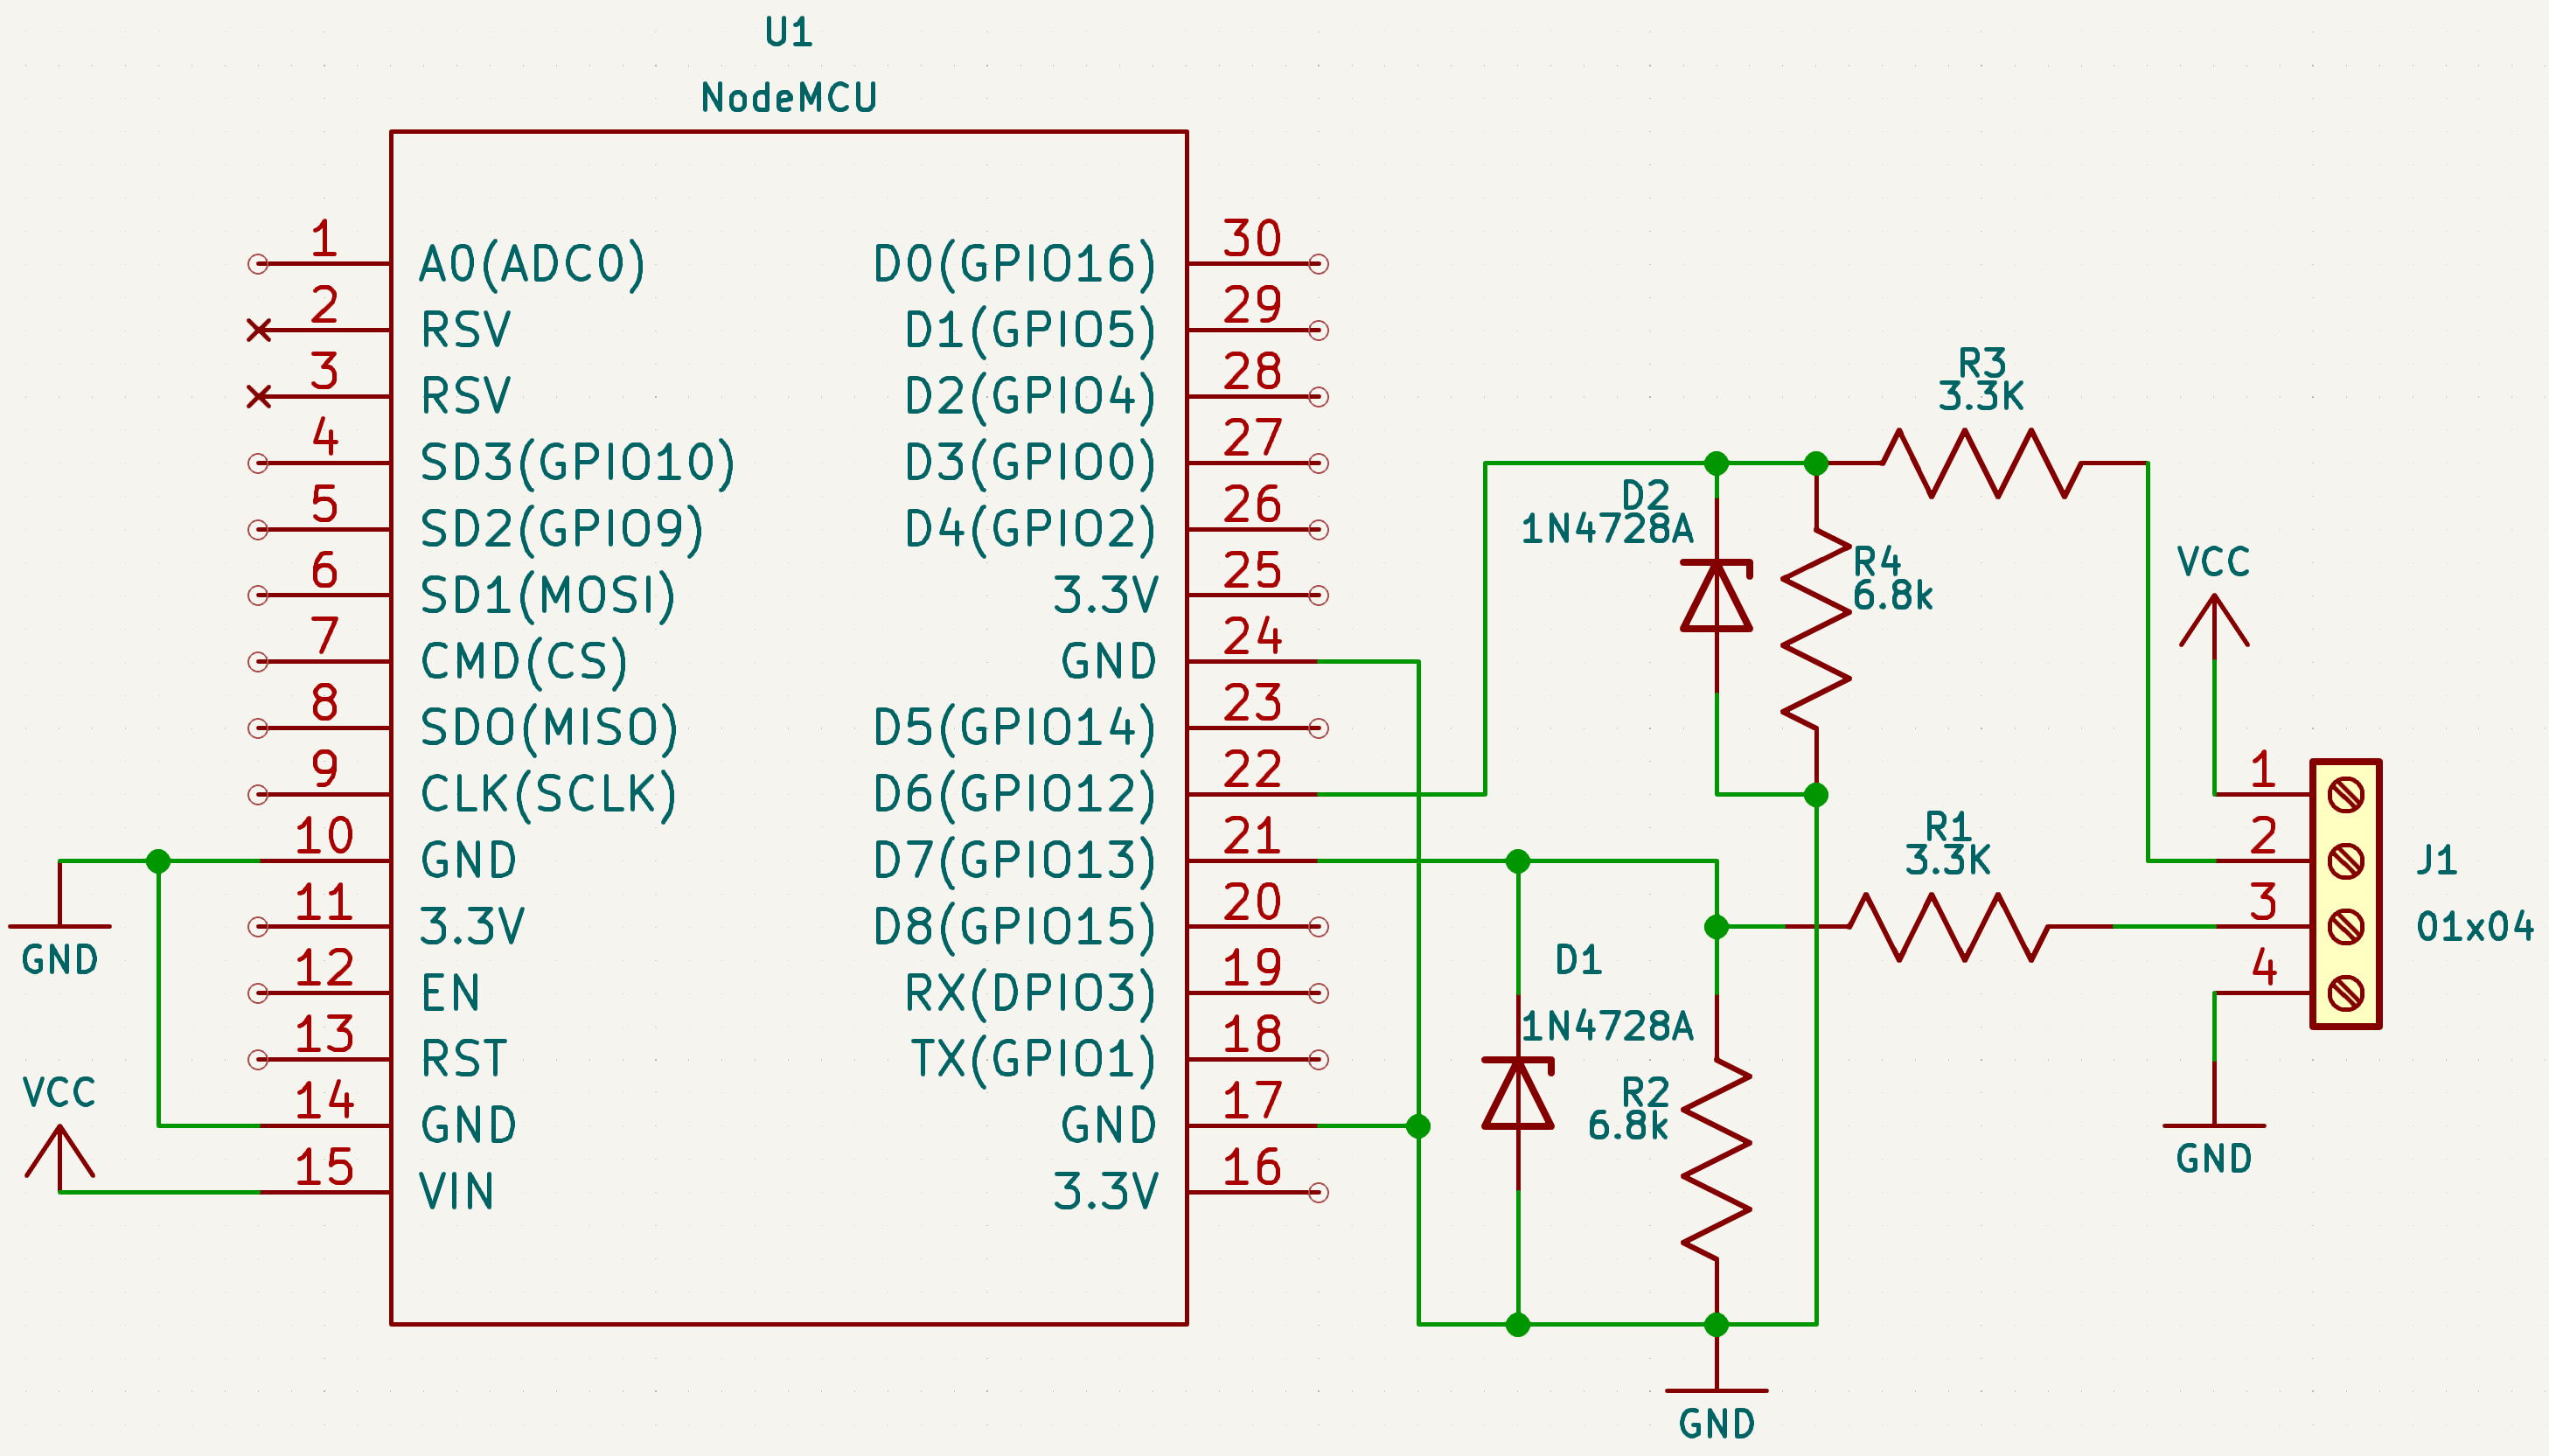
\includegraphics[width=\textwidth]{rfid-reader.png}
    \caption{RFID Reader}
    \label{fig:rfid-reader}
\end{figure}

